%%%%%%%%%%%%%%%%%%%%%%%%%%%%%%%%%%%%%%%%%
% Journal Article
% LaTeX Template
% Version 1.4 (15/5/16)
%
% This template has been downloaded from:
% http://www.LaTeXTemplates.com
%
% Original author:
% Frits Wenneker (http://www.howtotex.com) with extensive modifications by
% Vel (vel@LaTeXTemplates.com)
%
% License:
% CC BY-NC-SA 3.0 (http://creativecommons.org/licenses/by-nc-sa/3.0/)
%
%%%%%%%%%%%%%%%%%%%%%%%%%%%%%%%%%%%%%%%%%

%----------------------------------------------------------------------------------------
%	PACKAGES AND OTHER DOCUMENT CONFIGURATIONS
%----------------------------------------------------------------------------------------

\documentclass[twoside,twocolumn]{article}

\usepackage{blindtext} % Package to generate dummy text throughout this template

\usepackage[sc]{mathpazo} % Use the Palatino font
\usepackage[T1]{fontenc} % Use 8-bit encoding that has 256 glyphs
\linespread{1.05} % Line spacing - Palatino needs more space between lines
\usepackage{microtype} % Slightly tweak font spacing for aesthetics

\usepackage{amsmath}

\usepackage[english]{babel} % Language hyphenation and typographical rules

\usepackage[hmarginratio=1:1,top=32mm,columnsep=20pt]{geometry} % Document margins
\usepackage[hang, small,labelfont=bf,up,textfont=it,up]{caption} % Custom captions under/above floats in tables or figures
\usepackage{booktabs} % Horizontal rules in tables

\usepackage{lettrine} % The lettrine is the first enlarged letter at the beginning of the text

\usepackage[demo]{graphicx}

\usepackage{enumitem} % Customized lists
\setlist[itemize]{noitemsep} % Make itemize lists more compact

\usepackage{abstract} % Allows abstract customization
\renewcommand{\abstractnamefont}{\normalfont\bfseries} % Set the "Abstract" text to bold
\renewcommand{\abstracttextfont}{\normalfont\small\itshape} % Set the abstract itself to small italic text

\usepackage{titlesec} % Allows customization of titles
\renewcommand\thesection{\Roman{section}} % Roman numerals for the sections
\renewcommand\thesubsection{\roman{subsection}} % roman numerals for subsections
\titleformat{\section}[block]{\large\scshape\centering}{\thesection.}{1em}{} % Change the look of the section titles
\titleformat{\subsection}[block]{\large}{\thesubsection.}{1em}{} % Change the look of the section titles

\usepackage{fancyhdr} % Headers and footers
\pagestyle{fancy} % All pages have headers and footers
\fancyhead{} % Blank out the default header
\fancyfoot{} % Blank out the default footer
\fancyhead[C]{Quantum computation of Hubbard Model using IBM Q } % Custom header text
\fancyfoot[RO,LE]{\thepage} % Custom footer text

\usepackage{titling} % Customizing the title section

\usepackage{hyperref} % For hyperlinks in the PDF


%----------------------------------------------------------------------------------------
%	TITLE SECTION
%----------------------------------------------------------------------------------------

\setlength{\droptitle}{-4\baselineskip} % Move the title up

\pretitle{\begin{center}\Huge\bfseries} % Article title formatting
\posttitle{\end{center}} % Article title closing formatting
\title{Quantum computation of Hubbard Model using IBM Q} % Article title
\author{

}

\date{\today} % Leave empty to omit a date
\renewcommand{\maketitlehookd}{%
\begin{abstract}
\noindent
In this work are described the steps and the calculation results of the Hubbard Model
evolution using simulations and real runs on IBM Quantum processors. The Hubbard Model has been approached
considering hopping and interaction terms calculated separately, then the quantum circuit has beed developed
to simulate all Hamiltonian terms leveraging on IBM Quantum Experience.
\end{abstract}
}

%----------------------------------------------------------------------------------------

\begin{document}

% Print the title
\maketitle

%----------------------------------------------------------------------------------------
%	ARTICLE CONTENTS
%----------------------------------------------------------------------------------------

\section{Introduction}

\lettrine[nindent=0em,lines=3]{H}ubbard Model is an approximate model that can be used to described
interactive particles into a lattice, for example electrons interacting on a chain of atoms of a conductor or semiconductor.
The Hamiltonian describing the temporal evolution of this system is quite simple, as it is composed by a
kinetic (or hopping) term, describing the particle jumps between chain sites,
and by a potential (or interaction) term, describing the particle interactions on the same site.

In general, particles described by Hubbard Model can be either bosons or fermions: in this paper are considered the electrons
running on a chain of atoms, thus the particles considered are fermions.

The complete Hubbard Hamiltonian for electrons with spin interacting on a chain of atoms is an interesting model
that can be mapped into a quantum processor: the aim of this work is to map the complete Hubbard Hamiltonian on
IBM Q quantum simulator and real processors, considering spin interaction and dynamic of the system.

%------------------------------------------------

\section{The Hubbard Model}

The Hubbard Model temporal evolution is described by the following Hamiltonian:

\begin{equation}
\mathcal{H} = -t \sum_{<i,j>}^N{(\hat{b}^{\dagger}_i \hat{b}_j+\hat{b}^{\dagger}_j \hat{b}_i)}
+ V \sum_{i}^N{(\hat{n}_{i\uparrow}\hat{n}_{i\downarrow})}
\end{equation}

with $\hat{n}_{i\uparrow} = (\hat{b}^{\dagger}_i\hat{b}_i)_\uparrow$ and
$\hat{n}_{i\downarrow} = (\hat{b}^{\dagger}_i\hat{b}_i)_\downarrow$, and where $\hat{b}^{\dagger}_i$ and
$\hat{b}_j$ are respectively the fermionic creation operator in site $i$ and the fermionic annihilation
operator in site $j$, with $N$ the total sites number.

The $<i,j>$ means that just the neighbour nearest are selected, and $t$ and $V$ are respectively the hopping parameter and the spin interaction potential.

In case of 2 sites:

\begin{equation}
  \begin{aligned}
    \mathcal{H} & = -t (\hat{b}^{\dagger}_{1\uparrow}\hat{b}_{2\uparrow}+
    \hat{b}^{\dagger}_{2\uparrow}\hat{b}_{1\uparrow}+
    \hat{b}^{\dagger}_{1\downarrow}\hat{b}_{2\downarrow}+
    \hat{b}^{\dagger}_{2\downarrow}\hat{b}_{1\downarrow}) \\
    & + V(\hat{b}^{\dagger}_{1\uparrow}\hat{b}_{1\uparrow}\hat{b}^{\dagger}_{1\downarrow}\hat{b}_{1\downarrow}+
    \hat{b}^{\dagger}_{2\uparrow}\hat{b}_{2\uparrow}\hat{b}^{\dagger}_{2\downarrow}\hat{b}_{2\downarrow})
    \end{aligned}
  \end{equation}

Using a more compact notation:

\begin{equation}\label{eq:hamiltonian1}
\begin{aligned}
\mathcal{H} &= [-t \sum_\sigma (\hat{b}^{\dagger}_{1,\sigma}\hat{b}_{2,\sigma}+\hat{b}^{\dagger}_{2,\sigma}\hat{b}_{1,\sigma})]+\\
&+ [V \sum_i^2(\hat{n}_{i\downarrow}\hat{n}_{i\uparrow} + \hat{n}_{i\uparrow}\hat{n}_{i\downarrow})]
\end{aligned}
\end{equation}


The Hubbard Model Hamiltonian can be expressed highlighting the hopping and the interaction terms:

\begin{equation}
\mathcal{H} = \mathcal{H}_{hop} + \mathcal{H}_{int}
\end{equation}

In general, the hopping term is related to the movement of the particles through the atom chain, from site $1$ to site $2$,
while the interaction term defines the interaction of two particles with opposite spin into the same site.

%------------------------------------------------

\section{Hubbard Hamiltonian in spin notation}

In the next sections are performed the calculations of hopping and interaction terms of Hubbard Model Hamiltonian. In general, the following notation will be applied
to define lattice sites and electron spins:


\begin{equation}\label{eq:notation}
\begin{aligned}
\textcircled{\raisebox{-0.9pt}{1}}} \rightarrow Site~1,~spin~\uparrow \\
\textcircled{\raisebox{-0.9pt}{2}}} \rightarrow Site~1,~spin~\downarrow \\
\textcircled{\raisebox{-0.9pt}{3}}} \rightarrow Site~2,~spin~\uparrow \\
\textcircled{\raisebox{-0.9pt}{4}}} \rightarrow Site~2,~spin~\downarrow
\end{aligned}
\end{equation}

%------------------------------------------------

\subsection{Hopping term}

Consider the hopping Hamiltonian, it is possible to calculate the analytical expression:

\begin{equation}\label{eq:hopping}
\mathcal{H}_{hop} = -t \sum_{i,\sigma}^{N}{(\hat{b}^{\dagger}_{i,\sigma}\hat{b}_{i+1,\sigma}+h.c.)}
\end{equation}

we can perform a \textit{Fourier Transform} to find the Energy eigenvalues:

$$
\hat{b}_{j}=\sum_{k=1}^{\infty} e^{-ikj}\hat{b}_{k}
$$

$$
\hat{b}_{j+1}=\sum_{k=1}^{\infty} e^{-ik(j+1)}\hat{b}_{k}=\sum_{k=1}^{\infty} e^{-ikj+k}\hat{b}_{k}
$$

\begin{equation}
\begin{aligned}
\mathcal{H}_{hop} &= t\sum_{i,\sigma}^{N}{\sum_{k}(\hat{b}^{\dagger}_{k,\sigma}\hat{b}_{k',\sigma}e^{-i(k-k')j+k'}+\\
&+ \hat{b}^{\dagger}_{k+1,\sigma}\hat{b}_{k',\sigma}e^{-(-k+k')j+k})}
\end{aligned}
\end{equation}

Considering that $\sum_{j}e^{-i(k-k')j}=\delta(k-k')$ and applying the Eulero Identity, it is possible to obtain the hopping term analytical expression:

$$
\mathcal{H}_{hop} = 2t \sum_{i,\sigma}^{N}{cos(k) \,}\hat{b}^{\dagger}_{k,\sigma}\hat{b}_{k,\sigma}
$$

Now, starting from \ref{eq:hamiltonian1} it is possible to apply the \textit{Jordan-Wigner Transform}
to express the hopping term using spin notation. In general, the \textit{Jordan-Wigner Transform} maps
the fermionic operators $\hat{b}_i$ using spin states $S$, in particular with the notation
$\hat{b}^k_i \rightarrow S^+ e^{i\alpha_j}$ with $\alpha = \sum_i{(\hat{n}_i)}\pi$.

Thus, the spin creation operator in site $2$ and the spin annihilation operator in site $1$ are defined as:

\begin{equation}
\begin{aligned}
S^+_2 &= \mathbb{1} \otimes S^+\\
S^-_1 &= S^- \otimes \mathbb{1} \\
\end{aligned}
\end{equation}

as the particle is moving from site $1$ to site $2$, so it annihilates in site $1$ and recreates in site $2$.

In order to proceed with Hamiltonian expression, it's needed to discuss the commutation of some quantities:

\begin{equation}
\begin{aligned}
\{\hat{b}^\dagger_i,\hat{b}_j\} &= \delta_{i,j}\\
\{\hat{b}^\dagger_i,\hat{b}_i\} &= \{S^+_i,S^-_i\} = \mathbb{1}\\
\{S^+_2,S^-_1\} &= \{\mathbb{1},S^-\} \otimes \{S^-,\mathbb{1}\}\\
\{\sigma_z,S^+\} &= 0
\end{aligned}
\end{equation}

from which can be obtained:

\begin{equation}
\begin{aligned}
S^+_2 = \prod_{i=0}^{n_i \neq 0}{\sigma_z S^+_i}
\end{aligned}
\end{equation}

and

\begin{equation}\label{eq:b_chain}
\begin{aligned}
\hat{b}^\dagger = \prod_{j=0}^{i-1}{\sigma_z \cdots \sigma^+_j} \prod_{j=i+1}^n{\mathbb{1}}
\end{aligned}
\end{equation}

Using the described quantities, the terms of the equation \ref{eq:hopping} can be written as:

\begin{equation}
\begin{aligned}
\hat{b}^\dagger_1 \hat{b}_2 &= (\sigma^+ \otimes \mathbb{1}) \otimes (\sigma_z \otimes \sigma_z) =\\
&= -\sigma^- \otimes \sigma^-
\end{aligned}
\end{equation}

\begin{equation}
\begin{aligned}
\hat{b}^\dagger_2 \hat{b}_1 &= (\sigma_z \otimes \sigma^+) \otimes (\sigma^- \otimes \mathbb{1}) =\\
&= \sigma^+ \otimes \sigma^+
\end{aligned}
\end{equation}

where $\sigma^+ = \frac{\sigma_x+i\sigma_y}{2}$ and $\sigma^- = \frac{\sigma_x-i\sigma_y}{2}$.
Considering the relationships below

\begin{equation}
\begin{aligned}
\sigma^+ + \sigma^+ &= \sigma_x\\
\sigma^+ - \sigma^+ &= i\sigma_y
\end{aligned}
\end{equation}

the hopping term of the Hubbard Model Hamiltonian can be written using spin notation in this way:

\begin{equation} \label{eq:hopping_solution}
\mathcal{H}_{hop} = -\frac{t}{2}(\sigma_x \otimes \sigma_x + \sigma_y \otimes \sigma_y)
\end{equation}

Generalizing the $t$ parameter and applying the reference notation \ref{eq:notation}, it is possible to obtain the hopping term:

\begin{equation}\label{eq:hopping_solution2}
\begin{aligned}
\mathcal{H}_{hop} &= t [ (\sigma^x \otimes \mathbb{1} \otimes \sigma^x \otimes \mathbb{1}) \\
&+ (\sigma^y \otimes \mathbb{1} \otimes \sigma^y \otimes \mathbb{1}) +\\
&+ (\mathbb{1} \otimes \sigma^x \otimes \mathbb{1} \otimes \sigma^x) +\\
&+ (\mathbb{1} \otimes \sigma^y \otimes \mathbb{1} \otimes \sigma^y) ]
\end{aligned}
\end{equation}\\

%------------------------------------------------

\subsection{Interaction term}

The calculation of the interaction term of Hubbard Model Hamiltonian follows an approach similar to the hopping term.
Starting from the interaction term

\begin{equation}\label{eq:interaction_term}
\mathcal{H}_{int} = V{n_{i,\uparrow} n_{i,\downarrow}} = V(\hat{b}^\dagger_{i,\uparrow}\hat{b}_{i,\uparrow})(\hat{b}^\dagger_{i,\downarrow}\hat{b}_{i,\downarrow})
\end{equation}

and applying the notation \ref{eq:notation}
to get the structure of the interation in the position $j$,
it is possible to obtain a compact notation for the fermionic operators using pauli matrices:

\begin{equation}\label{eq:b+_chain}
\begin{aligned}
\hat{b}^\dagger_{\textcircled{\raisebox{-0.9pt}{1}}} \rightarrow \hat{b}^\dagger_{1,\uparrow} &=
  \sigma^+ \otimes \mathbb{1} \otimes \mathbb{1} \otimes \mathbb{1} \\
\hat{b}^\dagger_{\textcircled{\raisebox{-0.9pt}{2}}} \rightarrow \hat{b}^\dagger_{1,\downarrow} &=
  \sigma^z \otimes \sigma^+ \otimes \mathbb{1} \otimes \mathbb{1} \\
\hat{b}^\dagger_{\textcircled{\raisebox{-0.9pt}{3}}} \rightarrow \hat{b}^\dagger_{2,\uparrow} &=
  \sigma^z \otimes \sigma^z \otimes \sigma^+ \otimes \mathbb{1} \\
\hat{b}^\dagger_{\textcircled{\raisebox{-0.9pt}{4}}} \rightarrow \hat{b}^\dagger_{2,\downarrow} &=
  \sigma^z \otimes \sigma^z \otimes \sigma^z \otimes \sigma^+ \\
\end{aligned}
\end{equation}

\begin{equation}\label{eq:b_chain}
\begin{aligned}
\hat{b}_{\textcircled{\raisebox{-0.9pt}{1}}} \rightarrow \hat{b}^\dagger_{1,\uparrow} &=
  \sigma^- \otimes \mathbb{1} \otimes \mathbb{1} \otimes \mathbb{1} \\
\hat{b}_{\textcircled{\raisebox{-0.9pt}{2}}} \rightarrow \hat{b}^\dagger_{1,\downarrow} &=
  \sigma^z \otimes \sigma^- \otimes \mathbb{1} \otimes \mathbb{1} \\
\hat{b}_{\textcircled{\raisebox{-0.9pt}{3}}} \rightarrow \hat{b}^\dagger_{2,\uparrow} &=
  \sigma^z \otimes \sigma^z \otimes \sigma^- \otimes \mathbb{1} \\
\hat{b}_{\textcircled{\raisebox{-0.9pt}{4}}} \rightarrow \hat{b}^\dagger_{2,\downarrow} &=
  \sigma^z \otimes \sigma^z \otimes \sigma^z \otimes \sigma^- \\
\end{aligned}
\end{equation}

Applying \ref{eq:b+_chain} and \ref{eq:b_chain} to the terms of \ref{eq:interaction_term},
it is possible to obtain:

\begin{equation}
\begin{aligned}
\hat{b}^\dagger_{\textcircled{\raisebox{-0.9pt}{1}}}\hat{b}_{\textcircled{\raisebox{-0.9pt}{1}}} &=
  \frac{(\mathbb{1}+\sigma^z)}{2} \otimes \mathbb{1} \otimes \mathbb{1} \otimes \mathbb{1}\\
\hat{b}^\dagger_{\textcircled{\raisebox{-0.9pt}{2}}}\hat{b}_{\textcircled{\raisebox{-0.9pt}{2}}} &=
  \mathbb{1} \otimes \frac{(\mathbb{1}+\sigma^z)}{2} \otimes \mathbb{1} \otimes \mathbb{1}\\
\hat{b}^\dagger_{\textcircled{\raisebox{-0.9pt}{3}}}\hat{b}_{\textcircled{\raisebox{-0.9pt}{3}}} &=
  \mathbb{1} \otimes \mathbb{1} \otimes \frac{(\mathbb{1}+\sigma^z)}{2} \otimes \mathbb{1}\\
\hat{b}^\dagger_{\textcircled{\raisebox{-0.9pt}{4}}}\hat{b}_{\textcircled{\raisebox{-0.9pt}{4}}} &=
  \mathbb{1} \otimes \mathbb{1} \otimes \mathbb{1} \otimes \frac{(\mathbb{1}+\sigma^z)}{2}\\
\end{aligned}
\end{equation}

Considering the above formulas, the interaction term of Hubbard Model Hamiltonian can be written as:

$$
\mathcal{H}_{int} = V
  (\hat{b}^\dagger_{\textcircled{\raisebox{-0.9pt}{1}}}\hat{b}_{\textcircled{\raisebox{-0.9pt}{1}}})
  (\hat{b}^\dagger_{\textcircled{\raisebox{-0.9pt}{2}}}\hat{b}_{\textcircled{\raisebox{-0.9pt}{2}}}) (\hat{b}^\dagger_{\textcircled{\raisebox{-0.9pt}{3}}}\hat{b}_{\textcircled{\raisebox{-0.9pt}{3}}})
  (\hat{b}^\dagger_{\textcircled{\raisebox{-0.9pt}{4}}}\hat{b}_{\textcircled{\raisebox{-0.9pt}{4}}})
$$

\begin{equation}\label{eq:interaction_solution}
\begin{aligned}
\mathcal{H}_{int} &= V [ \mathbb{1} \otimes \mathbb{1} \otimes \mathbb{1} \otimes \mathbb{1} +\\
  &+ \sigma_z \otimes \sigma_z \otimes \mathbb{1} \otimes \mathbb{1} +\\
  &+ \mathbb{1} \otimes \mathbb{1} \otimes \sigma_z \otimes \sigma_z +\\
  &+ \sigma_z \otimes \mathbb{1} \otimes \mathbb{1} \otimes \mathbb{1} +\\
  &+ \mathbb{1} \otimes \sigma_z \otimes \mathbb{1} \otimes \mathbb{1} +\\
  &+ \mathbb{1} \otimes \mathbb{1} \otimes \sigma_z \otimes \mathbb{1} +\\
  &+ \mathbb{1} \otimes \mathbb{1} \otimes \mathbb{1} \otimes \sigma_z +\\
  &+ \mathbb{1} \otimes \mathbb{1} \otimes \mathbb{1} \otimes \mathbb{1} ]\\
\end{aligned}
\end{equation}

%------------------------------------------------

\subsection{Full spin Hamiltonian}

Combining the hopping term \ref{eq:hopping_solution2} and the interaction term \ref{eq:interaction_solution}
it is possible to write the full Hubbard Model Hamiltonian.

\begin{equation}\label{eq:hubb_hamiltonian_solution_full}
\begin{aligned}
\mathcal{H} &= \mathcal{H}_{hop} + \mathcal{H}_{int} = \\
&= t [ (\sigma^x \otimes \sigma^z \otimes \sigma^x \otimes \mathbb{1}) + (\sigma^y \otimes \sigma^z \otimes \sigma^y \otimes \mathbb{1}) +\\
&+ (\mathbb{1} \otimes \sigma^x \otimes \sigma^z \otimes \sigma^x) + (\mathbb{1} \otimes \sigma^y \otimes \sigma^z \otimes \sigma^y) ] +\\
&+ V [ (\mathbb{1} \otimes \mathbb{1} \otimes \mathbb{1} \otimes \mathbb{1}) + (\mathbb{1} \otimes \mathbb{1} \otimes \mathbb{1} \otimes \mathbb{1}) +\\
&+ (\sigma^z \otimes \sigma^z \otimes \mathbb{1} \otimes \mathbb{1}) + (\mathbb{1} \otimes \mathbb{1} \otimes \sigma^z \otimes \sigma^z) +\\
&+ (\sigma^z \otimes \mathbb{1} \otimes \mathbb{1} \otimes \mathbb{1}) + (\mathbb{1} \otimes \sigma^z \otimes \mathbb{1} \otimes \mathbb{1}) +\\
&+ (\mathbb{1} \otimes \mathbb{1} \otimes \sigma^z \otimes \mathbb{1}) + (\mathbb{1} \otimes \mathbb{1} \otimes \mathbb{1} \otimes \sigma^z) ]
\end{aligned}
\end{equation}\\

Optimized (no 3 body component)
\begin{equation}\label{eq:hubb_hamiltonian_solution_full}
\begin{aligned}
\mathcal{H} &= \mathcal{H}_{hop} + \mathcal{H}_{int} = \\
&= t [ (\sigma^x \otimes \mathbb{1} \otimes \sigma^x \otimes \mathbb{1}) + (\sigma^y \otimes \mathbb{1} \otimes \sigma^y \otimes \mathbb{1}) +\\
&+ (\mathbb{1} \otimes \sigma^x \otimes \mathbb{1} \otimes \sigma^x) + (\mathbb{1} \otimes \sigma^y \otimes \mathbb{1} \otimes \sigma^y) ] +\\
&+ V [ (\mathbb{1} \otimes \mathbb{1} \otimes \mathbb{1} \otimes \mathbb{1}) + (\mathbb{1} \otimes \mathbb{1} \otimes \mathbb{1} \otimes \mathbb{1}) +\\
&+ (\sigma^z \otimes \sigma^z \otimes \mathbb{1} \otimes \mathbb{1}) + (\mathbb{1} \otimes \mathbb{1} \otimes \sigma^z \otimes \sigma^z) +\\
&+ (\sigma^z \otimes \mathbb{1} \otimes \mathbb{1} \otimes \mathbb{1}) + (\mathbb{1} \otimes \sigma^z \otimes \mathbb{1} \otimes \mathbb{1}) +\\
&+ (\mathbb{1} \otimes \mathbb{1} \otimes \sigma^z \otimes \mathbb{1}) + (\mathbb{1} \otimes \mathbb{1} \otimes \mathbb{1} \otimes \sigma^z) ]
\end{aligned}
\end{equation}\\


Optimized (mapping 2)
\begin{equation}\label{eq:hubb_hamiltonian_solution_full}
\begin{aligned}
\mathcal{H} &= \mathcal{H}_{hop} + \mathcal{H}_{int} = \\
&= t [ (\sigma^x \otimes \sigma^x \otimes \mathbb{1} \otimes \mathbb{1}) + (\sigma^y \otimes \sigma^y \otimes \mathbb{1} \otimes \mathbb{1}) +\\
&+ (\mathbb{1} \otimes \mathbb{1} \otimes \sigma^x \otimes \sigma^x) + (\mathbb{1} \otimes \mathbb{1} \otimes \sigma^y \otimes \sigma^y) ] +\\
&+ V [ (\mathbb{1} \otimes \mathbb{1} \otimes \mathbb{1} \otimes \mathbb{1}) + (\mathbb{1} \otimes \mathbb{1} \otimes \mathbb{1} \otimes \mathbb{1}) +\\
&+ (\sigma^z \otimes \mathbb{1} \otimes \mathbb{1} \otimes \sigma^z) + (\mathbb{1} \otimes \sigma^z \otimes \sigma^z \otimes \mathbb{1}) +\\
&+ (\sigma^z \otimes \mathbb{1} \otimes \mathbb{1} \otimes \mathbb{1}) + (\mathbb{1} \otimes \sigma^z \otimes \mathbb{1} \otimes \mathbb{1}) +\\
&+ (\mathbb{1} \otimes \mathbb{1} \otimes \sigma^z \otimes \mathbb{1}) + (\mathbb{1} \otimes \mathbb{1} \otimes \mathbb{1} \otimes \sigma^z) ]
\end{aligned}
\end{equation}\\






\begin{figure}
  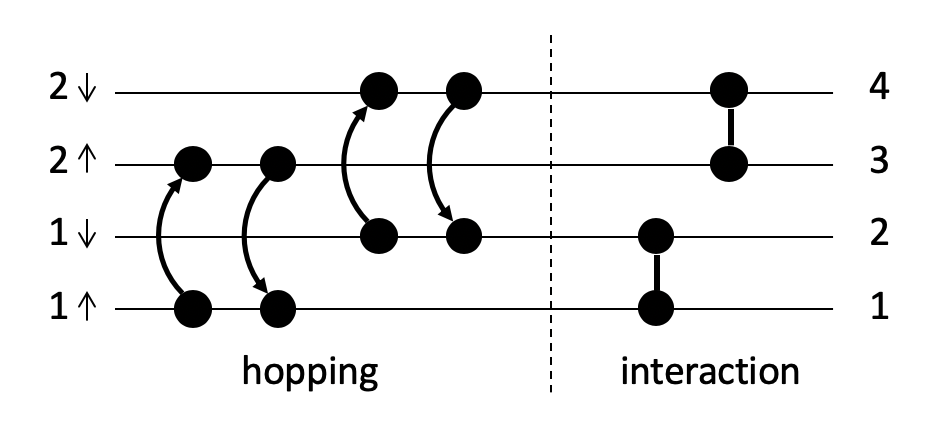
\includegraphics[width=\linewidth]{img/hamiltonian_terms.jpg}
  \caption{Hopping and interaction terms.}
  \label{fig:hamiltonian_terms}
\end{figure}


%------------------------------------------------

\section{Benchmark with analytical solution}

In order to check if the Hubbard Hamiltonian has been correctly expressed in spin notation, it is necessary to proceed with a benchmark: this is performed
expressing the time evolution (expressed with the notation $e^{-i\mathcal{H}t}$) of the system using both the exact analytical solution and the trotterized analytical solution.
In the first case, it is possible to perform a classical analytical calculation of time evolution of a system of two sites, using the notation
expressed in figure \ref{fig:hamiltonian_terms}.
In the second case, the same calculation can be performed considering the trotterization of the Hubbard Hamiltonian.

In the following figures is reported the benchmark results.\\

% INSERIRE GRAFICO TRA ANALITICA E ANALITICA TROTTERIZZATA CON IN DIDASCALIA I PARAMETRI E LO STATO INIZIALE

After verification of the spin translation of the Hubbard Hamiltonian \ref{eq:hubb_hamiltonian_solution_reduced} using the performed benchmarks,
the Hamiltonian expression \ref{eq:hubb_hamiltonian_solution_reduced} can be translated into a quantum circuit leveraging
on $4$ qubits, as the operators are mainly the basic IBM Q quantum gates. In the next section is described
the quantum algorithm creation.

%------------------------------------------------

\section{Hubbard quantum circuit}


In this section is reported the complete Hubbard hamiltonian to be implemented on the quantum processor. The first needed operation is to map the notation
expressed in \ref{eq:notation} on qubits, as the following relations:

\begin{equation}\label{eq:mapping}
\begin{aligned}
Qubit~0 \rightarrow \textcircled{\raisebox{-0.9pt}{1}}} \rightarrow Site~1,~spin~\uparrow \\
Qubit~1 \rightarrow \textcircled{\raisebox{-0.9pt}{2}}} \rightarrow Site~1,~spin~\downarrow \\
Qubit~2 \rightarrow \textcircled{\raisebox{-0.9pt}{3}}} \rightarrow Site~2,~spin~\uparrow \\
Qubit~3 \rightarrow \textcircled{\raisebox{-0.9pt}{4}}} \rightarrow Site~2,~spin~\downarrow
\end{aligned}
\end{equation}

The best form of Hubbard hamiltonian ready to be implemented on quantum processor is built from relation \ref{eq:hubb_hamiltonian_solution_full}:
here are not considered the trivial $\mathbb{1} \otimes \mathbb{1} \otimes \mathbb{1} \otimes \mathbb{1}$ terms,
and are specified the qubit involved on each operation, following the mapping \ref{eq:mapping}:


\begin{equation}\label{eq:hubb_hamiltonian_solution}
\begin{aligned}
\mathcal{H} &= \mathcal{H}_{hop} + \mathcal{H}_{int} = \\
&= \frac{t}{2} [ \sigma^x_{\textcircled{\raisebox{-0.9pt}{1}}} \otimes \sigma^x_{\textcircled{\raisebox{-0.9pt}{3}}}
  + \sigma^y_{\textcircled{\raisebox{-0.9pt}{1}}} \otimes \sigma^y_{\textcircled{\raisebox{-0.9pt}{3}}} ] + \\
&+ \frac{t}{2} [ \sigma^x_{\textcircled{\raisebox{-0.9pt}{2}}} \otimes \sigma^x_{\textcircled{\raisebox{-0.9pt}{4}}}
  + \sigma^y_{\textcircled{\raisebox{-0.9pt}{2}}} \otimes \sigma^y_{\textcircled{\raisebox{-0.9pt}{4}}} ] + \\
&+ V [\sigma^z_{\textcircled{\raisebox{-0.9pt}{1}}} \otimes \sigma^z_{\textcircled{\raisebox{-0.9pt}{2}}}
  \otimes \mathbb{1}_{\textcircled{\raisebox{-0.9pt}{3}}} \otimes \mathbb{1}_{\textcircled{\raisebox{-0.9pt}{4}}} ] +\\
&+ V [\mathbb{1}_{\textcircled{\raisebox{-0.9pt}{1}}} \otimes \mathbb{1}_{\textcircled{\raisebox{-0.9pt}{2}}}
  \otimes \sigma^z_{\textcircled{\raisebox{-0.9pt}{3}}} \otimes \sigma^z_{\textcircled{\raisebox{-0.9pt}{4}}} ] +\\
&+ V [\sigma^z_{\textcircled{\raisebox{-0.9pt}{1}}} \otimes \mathbb{1}_{\textcircled{\raisebox{-0.9pt}{2}}}
  \otimes \mathbb{1}_{\textcircled{\raisebox{-0.9pt}{3}}} \otimes \mathbb{1}_{\textcircled{\raisebox{-0.9pt}{4}}} ] +\\
&+ V [\mathbb{1}_{\textcircled{\raisebox{-0.9pt}{1}}} \otimes \sigma^z_{\textcircled{\raisebox{-0.9pt}{2}}}
  \otimes \mathbb{1}_{\textcircled{\raisebox{-0.9pt}{3}}} \otimes \mathbb{1}_{\textcircled{\raisebox{-0.9pt}{4}}} ] +\\
&+ V [\mathbb{1}_{\textcircled{\raisebox{-0.9pt}{1}}} \otimes \mathbb{1}_{\textcircled{\raisebox{-0.9pt}{2}}}
  \otimes \sigma^z_{\textcircled{\raisebox{-0.9pt}{3}}} \otimes \mathbb{1}_{\textcircled{\raisebox{-0.9pt}{4}}} ] +\\
&+ V [\mathbb{1}_{\textcircled{\raisebox{-0.9pt}{1}}} \otimes \mathbb{1}_{\textcircled{\raisebox{-0.9pt}{2}}}
  \otimes \mathbb{1}_{\textcircled{\raisebox{-0.9pt}{3}}} \otimes \sigma^z_{\textcircled{\raisebox{-0.9pt}{4}}}]\\
\end{aligned}
\end{equation}

The relationship \ref{eq:hubb_hamiltonian_solution} can be expressed in a more compact view,
excluding the trivial $\mathbb{1}_{\textcircled{\raisebox{-0.9pt}{i}}}$ terms:

\begin{equation}\label{eq:hubb_hamiltonian_solution_reduced}
\begin{aligned}
\mathcal{H} &= \mathcal{H}_{hop} + \mathcal{H}_{int} = \\
&= \frac{t}{2} [ \sigma^x_{\textcircled{\raisebox{-0.9pt}{1}}} \otimes \sigma^x_{\textcircled{\raisebox{-0.9pt}{3}}}
  + \sigma^y_{\textcircled{\raisebox{-0.9pt}{1}}} \otimes \sigma^y_{\textcircled{\raisebox{-0.9pt}{3}}} ] + \\
&+ \frac{t}{2} [ \sigma^x_{\textcircled{\raisebox{-0.9pt}{2}}} \otimes \sigma^x_{\textcircled{\raisebox{-0.9pt}{4}}}
  + \sigma^y_{\textcircled{\raisebox{-0.9pt}{2}}} \otimes \sigma^y_{\textcircled{\raisebox{-0.9pt}{4}}} ] + \\
&+ V [\sigma^z_{\textcircled{\raisebox{-0.9pt}{1}}} \otimes \sigma^z_{\textcircled{\raisebox{-0.9pt}{2}}} +
      \sigma^z_{\textcircled{\raisebox{-0.9pt}{3}}} \otimes \sigma^z_{\textcircled{\raisebox{-0.9pt}{4}}} ] +\\
&+ V [\sigma^z_{\textcircled{\raisebox{-0.9pt}{1}}} + \sigma^z_{\textcircled{\raisebox{-0.9pt}{2}}} +
      \sigma^z_{\textcircled{\raisebox{-0.9pt}{3}}} + \sigma^z_{\textcircled{\raisebox{-0.9pt}{4}}}]\\
\end{aligned}
\end{equation}


While a single $\sigma^z$ can be easily implemented on a quantum computer using a standard rotation among $z$-axis,
the implementation of $\sigma^x \otimes \sigma^x$, $\sigma^y \otimes \sigma^y$ and $\sigma^z \otimes \sigma^z$ require
the application of a transformation of the reference coordinate system. In particular, the relationships
used are the following:

\begin{equation}\label{eq:build_blocks}
\begin{aligned}
\hat{X} &\rightarrow [R_y(-\frac{\pi}{2}) \; Z \; R_y(\frac{\pi}{2})]\\
\hat{Y} &\rightarrow [R_x(-\frac{\pi}{2}) \; Z \; R_x(\frac{\pi}{2})]\\
\hat{Z}\hat{Z} &\rightarrow [CNOT \; R_z(2\delta) \; CNOT]
\end{aligned}
\end{equation}

where the parameter $\delta$ is the angle related to the temporal evolution of the system.
Using the "building blocks" reported in \ref{eq:build_blocks}, a quantum circuit describing the Hubbard Model hamiltonian
has been created, following the compact notation \ref{eq:hubb_hamiltonian_solution_reduced} with the qubit numbers in which to apply the quantum gates:

%----------------------------------------------------------------------------------------
%	REFERENCE LIST
%----------------------------------------------------------------------------------------

\begin{thebibliography}{99} % Bibliography - this is intentionally simple in this template

%\bibitem[Figueredo and Wolf, 2009]{Figueredo:2009dg}
%Figueredo, A.~J. and Wolf, P. S.~A. (2009).
%\newblock Assortative pairing and life history strategy - a cross-cultural study.
%\newblock {\em Human Nature}, 20:317--330.

\end{thebibliography}

%----------------------------------------------------------------------------------------

\end{document}
